\documentclass[journal=jpc]{achemso}
%\documentclass{article}
\usepackage{color}
\usepackage{graphicx}
\usepackage{amsmath}

\title{QTAG in the Libra Interface\\
\large{CyberTraining Workshop 2021 Project}}
\author{Matthew Dutra}
\email{dutramf@mailbox.sc.edu}
%\affiliation{Department of Chemistry and Biochemistry, University of South Carolina, Columbia, SC 29208, USA}

\begin{document}
\maketitle

The goals of this year's CyberTraining Workshop have primarily been twofold: to better understand the theory and concepts of nonadiabatic dynamics, and to share and train on software engineered to tackle problems in this field. With these overarching goals in mind, the aim of this project was to adapt the QTAG algorithm developed in the Garashchuk research group to interface with the Libra software package. This algorithm offers a means to study nuclear dynamics via a quantum trajectory-based approach, although its applications to date have been largely to multidimensional single-surface systems. This project, and indeed the workshop as a whole, has not only given us the resources to begin to expand the QTAG method to nonadiabatic systems, but also offered a means to improve its portability by connecting with Libra - thus aligning with both goals of the aforementioned workshop objectives.

In order to interface with Libra, the core of the QTAG algorithm - orignally coded in-house using the FORTRAN language - was reconstructed in Python 3.9. At present, it relies on the linear algebra, eigensolver, and Gaussian integration libraries found in Libra, although future iterations of this code could also take advantage of Libra's Hamiltonian and propagation routines. The workshop version of the QTAG algorithm is restricted to 1D systems with one or two surfaces; the particular model selected for this presentation is similar to the Holstein model, that is, two intersecting harmonic potentials with Gaussian coupling localized at the crossing region (Eqs. \ref{eq:pots} and Fig. \ref{fig:pots}). Note that this is a diabatic representation.

\begin{align}\label{eq:pots}
V_{11} & =  \frac{k_1}{2}x^2 \nonumber \\
V_{22} & =  \frac{k_2}{2}(x-x_0)^2 + y_0\\
V_{12}=V_{21} & =  d_1e^{-d_2(x-d_3)^2} \nonumber
\end{align}

\begin{figure}
\centering
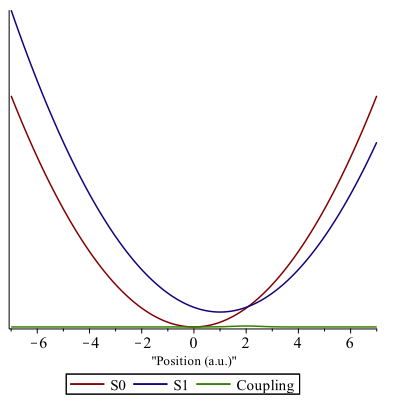
\includegraphics[angle=0,width=0.8\textwidth]{eps-files/potentials.png}
\caption{Diabatic potential curves for the selected 1D nonadiabatic model. S0 and S1 are of harmonic form, while the coupling is Gaussian.}
\label{fig:pots}
\end{figure}
\maketitle

Wavepacket dynamics were performed using 25 basis functions for a Gaussian wavepacket initially localized on the left side ($q_0=-2$ a.u.;$a_0=1.0$) of S0, propagated for up to $t=800$ a.u.; this duration was sufficient for multiple crossings into and out of the coupling region, as evidenced by the trajectory positions seen in Fig. \ref{fig:gbc-25}. The wavefunctions on both surfaces were reconstructed at $200$ a.u. intervals and compared with values calculated using the SOFT method; these results are displayed in Fig. \ref{fig:wf-25}.

\begin{figure}
\centering
\includegraphics[angle=-90,width=1.0\textwidth]{eps-files/gbc-800-09.eps}
\caption{Quantum trajectories over the course of $t=800$ a.u. on the ground (black) and first excited(red) states (overlaid). The horizontal line at $x=2.0$ indicates the center of the coupling region. Note that the periodicity for this there-and-back motion is $\approx200$ a.u.}
\label{fig:gbc-25}
\end{figure}
\maketitle

\begin{figure}
\centering
\includegraphics[angle=-90,width=1.0\textwidth]{eps-files/wfs-25-09.eps}
\caption{Snapshots of |$\Psi(x)$| on the ground (black) and first excited (red) states over the course of the dynamics. Solid lines = QTAG; points = SOFT.}
\label{fig:wf-25}
\end{figure}
\maketitle

The agreement between the QTAG and SOFT wavefunctions is quite good for the first $t=400$ a.u., i.e. for two periods of the wavefunction oscillation in the ground state. However, error accumulates over the course of the simulation, and discrepancies due to edge effects can be seen at later times (although the general contour of the wavefunctions on each surface are preserved). The populations on each surface - computed as the integrals over each density $\rho_1(x)$ and $\rho_2(x)$ - also agree with SOFT values (a visual is not given presently); in particular, each period of oscillation from $t=0$ to $t=600$ a.u. results in approximately 20\% of the density being transferred from the ground to the excited state. 

While encouraging, the selected model also represents a scenario in which the QTAG method is expected to perform well: the potential elements for both surfaces and their coupling can be computed analytically, a benefit that doesn't hold true for many sets of other potentials. An interesting follow-up will be calculations using the Tully models, which feature surfaces whose matrix elements will have to be computed within the local harmonic approximation. Another avenue to explore will be the implementation of surface-hopping techniques to the QTAG algorithm - such methods have been successful in the past, employing classical trajectories, although their adaptation to the present work is not straightforward. In particular, it is challenging to build a wavefunction on an initially unpopulated surface through hopping when the trajectory dynamics themselves depend upon the phase gradient of said wavefunction.


\end{document}